%-----------------------------------------------------
\begin{frame}
\frametitle{EGO en pratique : deux points critiques (1/2)}

\begin{block}{1- Maximisation de l'amélioration espérée}
\begin{itemize}
 \item Sous-problème d'optimisation (globale) difficile !
 \item $EI$ ``gratuit'' ($\approx 1/100s$) $\rightarrow$ méthodes intensives
 \item De plus : gradients et hessiens analytiques
\end{itemize}
\end{block}

\begin{columns}
 \begin{column}{.5\textwidth}

\begin{figure}[h!]  \centering	
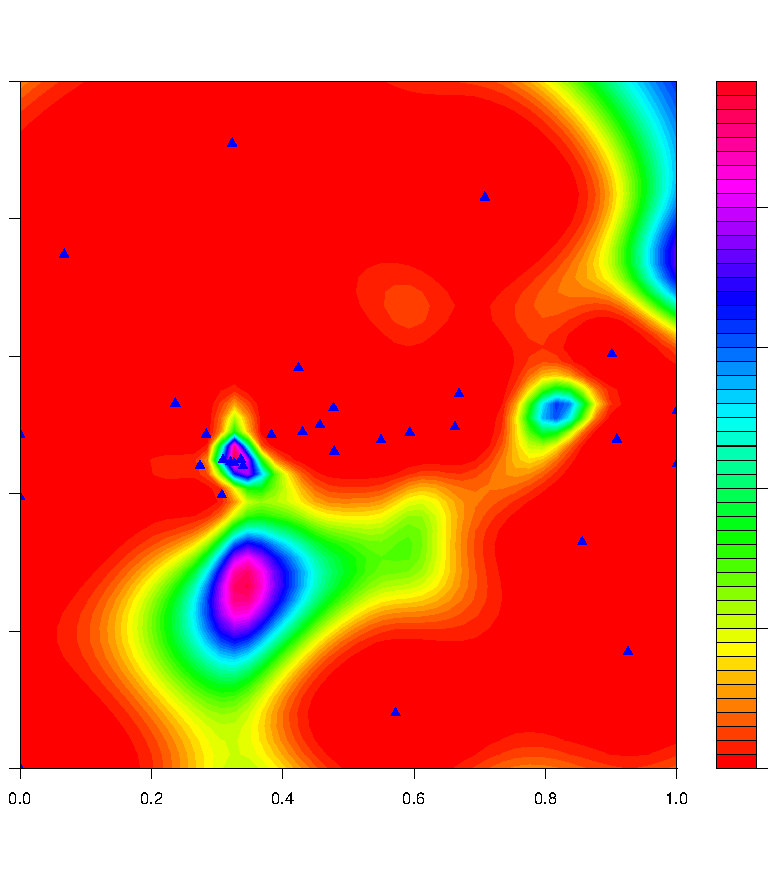
\includegraphics[trim=1mm 15mm 20mm 20mm, clip, width=.7\textwidth]{fig/AEI.png} 
\end{figure}  
 \end{column}
 \begin{column}{.5\textwidth}
\begin{block}{cf. R package \texttt{DiceOptim}}
\scriptsize{
 \begin{thebibliography}{7}
\beamertemplatearticlebibitems
     \bibitem{dkdo}
     O.~Roustant D.~Ginsbourger, Y.~Deville (2010)
         \newblock DiceKriging, DiceOptim: Two R packages for the analysis of computer experiments by kriging-based metamodeling and optimization  
         \newblock Journal of Computational Software
 \end{thebibliography}
}
\end{block}
 \end{column}
\end{columns}
\end{frame}

%-----------------------------------------------------
\begin{frame}
\frametitle{EGO en pratique : deux points critiques (2/2)}

\begin{block}{2- Apprentissage du modèle de krigeage}
\begin{itemize}
 \item Quelle proportion plan initial / optimisation ?
 \item Choix a priori du modèle
 \item Paramètres de covariance : ré-estimation ?
 \begin{itemize}
   \item coûteux $\rightarrow$ dépend du temps de calcul pour une simulation !
   \item parfois instable
  \end{itemize}
\end{itemize}
\end{block}

\begin{block}{Quelques résultats... à prendre avec précaution}
\scriptsize{
 \begin{thebibliography}{7}
\beamertemplatearticlebibitems
     \bibitem{dkdo}
     Picheny, Wagner, Ginsbourger (2013)
         \newblock A benchmark of kriging-based infill criteria for noisy optimization
         \newblock Structural and Multidisciplinary Optimization
 \end{thebibliography}
}
\normalsize
\begin{itemize}
 \item Budget du plan initial (20\% - 50\%) \& choix du noyau : peu critiques
 \item \textcolor{red}{Paramètres de covariance \& capacité du modèle à représenter la fonction : influence majeure sur le comportement !}
\end{itemize}
\end{block}
\end{frame}